
\section{The 487 potentially prime spaces in $U$}
\label{chap:primeCatalogue}

We present in this chapter the 487 spaces that are ``potentially prime'' once we could
not prove them composite in our tests. One thing is certain, as stated in
Theorem~\ref{theo:primeSpacesUpTo9Edges}: any prime space that can be
presented as a blink with $\leq$ 9 edges induces the same space (modulo
orientation) as one and only one of these 487 spaces. Actually there
are two points where this last statement may fail: space 9.126 and space 9.199 (although
they have the same HGnQI we could not find a proof of homeomorphism
between g-blink $U[1563]$ and the other g-blinks in 9.126 and g-blink $U[2165]$
and the others in 9.199). All 3437 g-blinks in $U$ appears in this Appendix or
in Appendix~\ref{chap:compositeCatalogue}.

\begin{figure}[htp]
   \begin{center}
      \leavevmode
      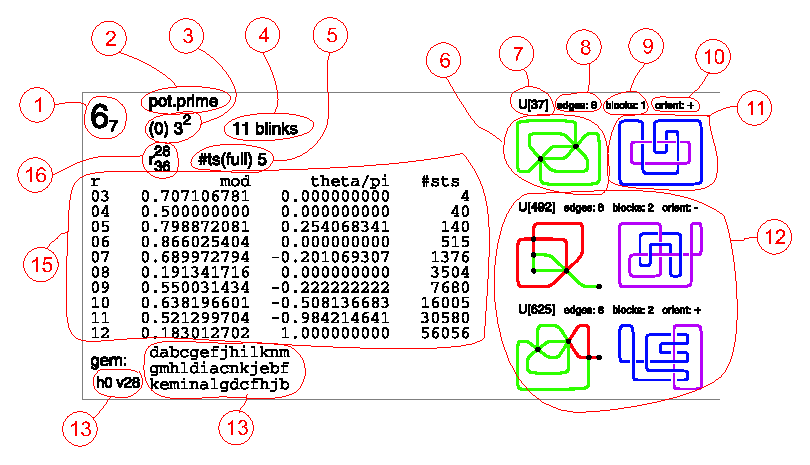
\includegraphics[width=14.5cm]{A.figs/catalogueexplanation.eps}
   \end{center}
   \vspace{-0.7cm}
   \caption{ Elements of catalogue}
   \label{fig:catalogueExplanation}
\end{figure}

The elements of this catalogue are: (1) the space name: $6_7$ is
a synonym for $6.7$; (2) the primality test outcome; (3) the homology
group; (4) the number of g-blinks in $U$ that induces this space; (5) number
of 3-gems identified in the same ts-class of the minimum 3-gem
found for this space: {\it full} means that all ts-class
was identified, {\it partial} means that we do not know if
all ts-class was identified; (6) the minimum blink
presentation for this space in set $U$ and also a
minimal presentation for this space (this is always true,
except for class $6.5$ that should be $0.1$); (7) the name
of the g-blink in $U$; (8) its number of edges; (9) its number
of blocks in the blink presentation (2-connected components);
(10) its orientation compared to the orientation of the QI shown:
+ sign means the same and - sign means different; (11) the
corresponding BFL presentation; (12) other g-blinks in the
same space; (13) the code of the minimal 3-gem found for
this space the code convention is defined in \cite{Lins1995};
 (14) the number of handles (composition with
$S^2 \times S^1$ and the number of vertices of this 3-gem); (15)
the quantum invariant of this space in polar form where the
angle is divided by $\pi$; (16) the name of this minimal
3-gem in the catalogue of \cite{Lins1995} when it is present
in this catalogue.

The spaces that have integral quantum invariants up to level 12 are:
6.5 $(S^2 \times S^1)$, 6.8, 6.18 and 8.32. The spaces that have real but not integral
quantum invariant up to level 12 are 1.1, 2.1, 4.4, 6.14, 6.19, 8.58,
8.70, 8.75, 8.76, 8.81, 8.86, 8.87, 8.89, 8.100, 8.102, 8.103, 8.117,
9.23, 9.183. The remaining classes have entries with non-zero imaginary
part (i.e. $\theta/\pi \notin \{0, 1\}$).



\begin{center}
 \includegraphics[height=23.5cm]{E.figsbw2/catalog001_bw.pdf} \eject
 \includegraphics[height=23.5cm]{E.figsbw2/catalog002_bw.pdf} \eject
 \includegraphics[height=23.5cm]{E.figsbw2/catalog003_bw.pdf} \eject
 \includegraphics[height=23.5cm]{E.figsbw2/catalog004_bw.pdf} \eject
 \includegraphics[height=23.5cm]{E.figsbw2/catalog005_bw.pdf} \eject
 \includegraphics[height=23.5cm]{E.figsbw2/catalog006_bw.pdf} \eject
 \includegraphics[height=23.5cm]{E.figsbw2/catalog007_bw.pdf} \eject
 \includegraphics[height=23.5cm]{E.figsbw2/catalog008_bw.pdf} \eject
 \includegraphics[height=23.5cm]{E.figsbw2/catalog009_bw.pdf} \eject
 \includegraphics[height=23.5cm]{E.figsbw2/catalog010_bw.pdf} \eject
 \includegraphics[height=23.5cm]{E.figsbw2/catalog011_bw.pdf} \eject
 \includegraphics[height=23.5cm]{E.figsbw2/catalog012_bw.pdf} \eject
 \includegraphics[height=23.5cm]{E.figsbw2/catalog013_bw.pdf} \eject
 \includegraphics[height=23.5cm]{E.figsbw2/catalog014_bw.pdf} \eject
 \includegraphics[height=23.5cm]{E.figsbw2/catalog015_bw.pdf} \eject
 \includegraphics[height=23.5cm]{E.figsbw2/catalog016_bw.pdf} \eject
 \includegraphics[height=23.5cm]{E.figsbw2/catalog017_bw.pdf} \eject
 \includegraphics[height=23.5cm]{E.figsbw2/catalog018_bw.pdf} \eject
 \includegraphics[height=23.5cm]{E.figsbw2/catalog019_bw.pdf} \eject
 \includegraphics[height=23.5cm]{E.figsbw2/catalog020_bw.pdf} \eject
 \includegraphics[height=23.5cm]{E.figsbw2/catalog021_bw.pdf} \eject
 \includegraphics[height=23.5cm]{E.figsbw2/catalog022_bw.pdf} \eject
 \includegraphics[height=23.5cm]{E.figsbw2/catalog023_bw.pdf} \eject
 \includegraphics[height=23.5cm]{E.figsbw2/catalog024_bw.pdf} \eject
 \includegraphics[height=23.5cm]{E.figsbw2/catalog025_bw.pdf} \eject
 \includegraphics[height=23.5cm]{E.figsbw2/catalog026_bw.pdf} \eject
 \includegraphics[height=23.5cm]{E.figsbw2/catalog027_bw.pdf} \eject
 \includegraphics[height=23.5cm]{E.figsbw2/catalog028_bw.pdf} \eject
 \includegraphics[height=23.5cm]{E.figsbw2/catalog029_bw.pdf} \eject
 \includegraphics[height=23.5cm]{E.figsbw2/catalog030_bw.pdf} \eject
 \includegraphics[height=23.5cm]{E.figsbw2/catalog031_bw.pdf} \eject
 \includegraphics[height=23.5cm]{E.figsbw2/catalog032_bw.pdf} \eject
 \includegraphics[height=23.5cm]{E.figsbw2/catalog033_bw.pdf} \eject
 \includegraphics[height=23.5cm]{E.figsbw2/catalog034_bw.pdf} \eject
 \includegraphics[height=23.5cm]{E.figsbw2/catalog035_bw.pdf} \eject
 \includegraphics[height=23.5cm]{E.figsbw2/catalog036_bw.pdf} \eject
 \includegraphics[height=23.5cm]{E.figsbw2/catalog037_bw.pdf} \eject
 \includegraphics[height=23.5cm]{E.figsbw2/catalog038_bw.pdf} \eject
 \includegraphics[height=23.5cm]{E.figsbw2/catalog039_bw.pdf} \eject
 \includegraphics[height=23.5cm]{E.figsbw2/catalog040_bw.pdf} \eject
 \includegraphics[height=23.5cm]{E.figsbw2/catalog041_bw.pdf} \eject
 \includegraphics[height=23.5cm]{E.figsbw2/catalog042_bw.pdf} \eject
 \includegraphics[height=23.5cm]{E.figsbw2/catalog043_bw.pdf} \eject
 \includegraphics[height=23.5cm]{E.figsbw2/catalog044_bw.pdf} \eject
 \includegraphics[height=23.5cm]{E.figsbw2/catalog045_bw.pdf} \eject
 \includegraphics[height=23.5cm]{E.figsbw2/catalog046_bw.pdf} \eject
 \includegraphics[height=23.5cm]{E.figsbw2/catalog047_bw.pdf} \eject
 \includegraphics[height=23.5cm]{E.figsbw2/catalog048_bw.pdf} \eject
 \includegraphics[height=23.5cm]{E.figsbw2/catalog049_bw.pdf} \eject
 \includegraphics[height=23.5cm]{E.figsbw2/catalog050_bw.pdf} \eject
 \includegraphics[height=23.5cm]{E.figsbw2/catalog051_bw.pdf} \eject
 \includegraphics[height=23.5cm]{E.figsbw2/catalog052_bw.pdf} \eject
 \includegraphics[height=23.5cm]{E.figsbw2/catalog053_bw.pdf} \eject
 \includegraphics[height=23.5cm]{E.figsbw2/catalog054_bw.pdf} \eject
 \includegraphics[height=23.5cm]{E.figsbw2/catalog055_bw.pdf} \eject
 \includegraphics[height=23.5cm]{E.figsbw2/catalog056_bw.pdf} \eject
 \includegraphics[height=23.5cm]{E.figsbw2/catalog057_bw.pdf} \eject
 \includegraphics[height=23.5cm]{E.figsbw2/catalog058_bw.pdf} \eject
 \includegraphics[height=23.5cm]{E.figsbw2/catalog059_bw.pdf} \eject
 \includegraphics[height=23.5cm]{E.figsbw2/catalog060_bw.pdf} \eject
 \includegraphics[height=23.5cm]{E.figsbw2/catalog061_bw.pdf} \eject
 \includegraphics[height=23.5cm]{E.figsbw2/catalog062_bw.pdf} \eject
 \includegraphics[height=23.5cm]{E.figsbw2/catalog063_bw.pdf} \eject
 \includegraphics[height=23.5cm]{E.figsbw2/catalog064_bw.pdf} \eject
 \includegraphics[height=23.5cm]{E.figsbw2/catalog065_bw.pdf} \eject
 \includegraphics[height=23.5cm]{E.figsbw2/catalog066_bw.pdf} \eject
 \includegraphics[height=23.5cm]{E.figsbw2/catalog067_bw.pdf} \eject
 \includegraphics[height=23.5cm]{E.figsbw2/catalog068_bw.pdf} \eject
 \includegraphics[height=23.5cm]{E.figsbw2/catalog069_bw.pdf} \eject
 \includegraphics[height=23.5cm]{E.figsbw2/catalog070_bw.pdf} \eject
 \includegraphics[height=23.5cm]{E.figsbw2/catalog071_bw.pdf} \eject
 \includegraphics[height=23.5cm]{E.figsbw2/catalog072_bw.pdf} \eject
 \includegraphics[height=23.5cm]{E.figsbw2/catalog073_bw.pdf} \eject
 \includegraphics[height=23.5cm]{E.figsbw2/catalog074_bw.pdf} \eject
 \includegraphics[height=23.5cm]{E.figsbw2/catalog075_bw.pdf} \eject
 \includegraphics[height=23.5cm]{E.figsbw2/catalog076_bw.pdf} \eject
 \includegraphics[height=23.5cm]{E.figsbw2/catalog077_bw.pdf} \eject
 \includegraphics[height=23.5cm]{E.figsbw2/catalog078_bw.pdf} \eject
 \includegraphics[height=23.5cm]{E.figsbw2/catalog079_bw.pdf} \eject
 \includegraphics[height=23.5cm]{E.figsbw2/catalog080_bw.pdf} \eject
 \includegraphics[height=23.5cm]{E.figsbw2/catalog081_bw.pdf} \eject
 \includegraphics[height=23.5cm]{E.figsbw2/catalog082_bw.pdf} \eject
 \includegraphics[height=23.5cm]{E.figsbw2/catalog083_bw.pdf} \eject
 \includegraphics[height=23.5cm]{E.figsbw2/catalog084_bw.pdf} \eject
 \includegraphics[height=23.5cm]{E.figsbw2/catalog085_bw.pdf} \eject
 \includegraphics[height=23.5cm]{E.figsbw2/catalog086_bw.pdf} \eject
 \includegraphics[height=23.5cm]{E.figsbw2/catalog087_bw.pdf} \eject
 \includegraphics[height=23.5cm]{E.figsbw2/catalog088_bw.pdf} \eject
 \includegraphics[height=23.5cm]{E.figsbw2/catalog089_bw.pdf} \eject
 \includegraphics[height=23.5cm]{E.figsbw2/catalog090_bw.pdf} \eject
 \includegraphics[height=23.5cm]{E.figsbw2/catalog091_bw.pdf} \eject
 \includegraphics[height=23.5cm]{E.figsbw2/catalog092_bw.pdf} \eject
 \includegraphics[height=23.5cm]{E.figsbw2/catalog093_bw.pdf} \eject
 \includegraphics[height=23.5cm]{E.figsbw2/catalog094_bw.pdf} \eject
 \includegraphics[height=23.5cm]{E.figsbw2/catalog095_bw.pdf} \eject
 \includegraphics[height=23.5cm]{E.figsbw2/catalog096_bw.pdf} \eject
 \includegraphics[height=23.5cm]{E.figsbw2/catalog097_bw.pdf} \eject
 \includegraphics[height=23.5cm]{E.figsbw2/catalog098_bw.pdf} \eject
 \includegraphics[height=23.5cm]{E.figsbw2/catalog099_bw.pdf} \eject
 \includegraphics[height=23.5cm]{E.figsbw2/catalog100_bw.pdf} \eject 
 \includegraphics[height=23.5cm]{E.figsbw2/catalog101_bw.pdf} \eject
\end{center}



